\graphicspath{{chapters/06/}}
\chapter{Atomic physics}
\section{Quantum theory of the Hydrogen atom}
\subsection{Evaluation of conservation of energy}
Remember that when talking about classical theory of the hydrogen atom we simplified the problem by switching from Cartesian to polar coordinates and, by applying the conservation laws, we obtained:
\[
E=\frac{1}{2}m\bigg(\frac{d}{dt}n\bigg)^2+\frac{L^2}{2mr^2}+U(r)
\]
that can be represented in quantum mechanics with the hamiltonian. The hamiltonian in polar coordinates is written as
\[
\hat{H}=(-\frac{\hbar^2}{2m^2}\, \nabla - \frac{e^2}{r})
\]
The best evaluation of the hamiltonian for the quantum analysis of the hydrogen atom is obtained by using the \textbf{spherical coordinates}. Nabla (the Laplacian) in spherical coordinates $(r,\theta,\varphi)$ is hence written as:
\[
\nabla^2=\frac{1}{r^2}\frac{\partial^2}{\partial r^2}+\frac{1}{r^2}\cdot\bigg(\frac{\partial^2}{\partial \theta^2}+\frac{1}{\tan\theta}\frac{\partial}{\partial\theta}+\frac{1}{\sin\theta}\frac{\partial^2}{\partial\varphi^2}\bigg)
\]
The hamiltonian so becomes:
\[
\hat{H}=\frac{\hbar^2}{2mr^2}\frac{\partial^2}{\partial r^2}+\frac{\hbar^2}{2mr^2}\cdot\bigg(\frac{\partial^2}{\partial \theta^2}+\frac{1}{\tan\theta}\frac{\partial}{\partial\theta}+\frac{1}{\sin\theta}\frac{\partial^2}{\partial\varphi^2}\bigg)-\frac{e^2}{r}
\]
The first part is called \textbf{radial part} because it's $r$-dependent only, the other is the \textbf{angular part} and depends on $r$, $\theta$, and $\varphi$.\\
Now we can consider the angular momentum in classical mechanics and quantum mechanics:
\[
\vec{L}=\vec{r}\times\vec{p}=\vec{r}\times(-i\vec{\nabla}\hbar)
\]
\[
\textit{Fact} \rightarrow \vec{\hat{L^2}}=\hat{L_x}\hat{L_x}+\hat{L_y}\hat{L_y}+\hat{L_z}\hat{L_z}=\vec{\nabla}^2\hbar^2
\]
This is corresponding to the angular part of the hamiltonian that can be rewritten in sperical coordinates with the inclusion of the angular momentum multiplied by $\hbar^2$.
\[
\hat{H}=\frac{\hbar^2}{2mr^2}\frac{\partial^2}{\partial r^2}+\frac{\hat{L^2}}{2mr^2}-\frac{e^2}{r}
\]
The fact that the angular momentum is not present in the radial part of the hamiltonian means that the two operators must commute $[\hat{H},\,\hat{L^2}]=0$ and they must also share the same eigenstates. It's also important to note that the invidual components of the angular momentum only commute with $\hat{L^2}$ but not with each other.\\
\[
\begin{cases}
[\hat{L_i},\,\hat{L_j}]\neq0 & i,j=1, 2, 3, ...\\
[\hat{L_i},\,\hat{L^2}]=0
\end{cases}
\]
\\
The following functions are called \textbf{spherical harmonics}, these functions are defined on the surface of a sphere and form a complete and orthonormal set of functions. For this latter reason they can be expressed as a linear combination. In quantum mechanics, spherical harmonics are the eigenfunctions of $\hat{L}^2$ and actually generate a rotation of azimuthal angle ($\varphi$). They depend on two quantum numbers because they use two different operators and are only part of the angular part of the hamiltonian.\\
\[
\begin{cases}
\hat{L_z}Y_{lm}(\theta,\varphi)=\hbar mY_{l,m}(\theta,\varphi) & m = l, -l+1,..., 0,..., -l \,\text{(projection)}\\
\hat{L^2}Y_{lm}(\theta,\varphi)=\hbar^2 l(l+1)Y_{l,m}(\theta,\varphi) & l = 0, 1, 2, ... \,\text{(max length,)}\, m < l^2
\end{cases}
\]
\textbf{N.B.:} in this way we obtain the quantization of $\hat{L_j}$ and $\hat{L^2}$.\\
Where $m$ represents the projection (bounded to $l$), and $l$ the length. Note that we wrote $l(l+1)$ and not $l^2$, the difference only matters in the quantum realm and it is noticeable when $l$ is small. For larger $l$ we go back to the classical realm (correspondence principle).\\
The wave function can then undergo variables separation, this implies the fact that eigenstates of the hamiltonian are also eigenstates of the square of the angular momentum.
\[
\Psi_{n,l,m}(r,\theta,\varphi)=R(r)\cdot Y_{l,m}(\theta,\varphi)
\]
I can calculate the hamiltonian of the newly obtained wave function.
\[
\hat{H}\psi_{n,l,m}=\bigg[\frac{-\hbar^2}{2mr^2}\frac{\partial^2r}{\partial r^2}R_nY_{l,m}+\frac{\hbar^2l(l+1)}{2mr^2}R_nY_{l,m}-\frac{e^2}{r}R_nY_{l,m}\bigg]=E_{n,m,l}R_nY_{l,m}
\]
By eliminating $Y_{l,m}$ we obtain the \textbf{one-dimensional Schr\"odinger equation}, I obtain one equation for each value of $l$. Each equation is referred to a different expression of energy.
\[
\frac{-\hbar^2}{2mr^2}\frac{\partial^2r}{\partial r^2}R_n+\frac{\hbar^2l(l+1)}{2mr^2}R_n-\frac{e^2}{r}R_n=E_{n,m,l}R_n
\]
\\

\subsection{Angular momentum conservation}
We can also rewrite kinetic energy in a polar form.\\
\[
-\frac{\hbar^2}{2m}\nabla^2 \rightarrow-\frac{\hbar^2}{2m}\frac{1}{r}\frac{\partial^2}{\partial r^2}\dot{r}+\frac{\hat{L^2}}{2mr^2} = \hat{T_r}+\hat{T}_{(\theta,\varphi)}
\]
Where $\hat{T_r}$ is the radial component of kinetic energy, $\hat{T}_{(\theta,\varphi)}$ is the angular component of kinetic energy. Note that if the radial part is applied to a radial function $rR(r)$, the second derivative applies to the product of $r$ and the function, not just to $r$.
\[
R(r)=\frac{1}{r}\frac{\partial^2(r\cdot R(r))}{\partial r^2}
\]
As we said before, the hamiltonian commutes with the square of the angular momentum $[\hat{H},\,\hat{L^2}]=0$ because the angular momentum doesn't have any derivatives with respect to $r$. By considering the hamiltonian as $\hat{H}=\hat{T_r}+\hat{V}$ with $\hat{V}$ as describing the coulomb potential, these commutations are possible:\\
\[
[\hat{T_r}\,,\,\hat{L^2}]=0\,,\,\,\,[\hat{V}\,,\,\hat{L}]=0\,,\,\,\,[\hat{L^2}\,,\,\hat{L^2}]=0
\]
All these have common sets of eigenstates. Note that $\hat{T_r}\,,\,\hat{L^2}]=0$ is possible beacuse $\hat{T_r}$ doesn't depened on $\theta$ \\
\newline
We can implement the fact that the operators, as said above, share a common set of eigenstate by pluggin the following:
\[
\psi_{nml}(r, \theta, \varphi) = R_n(r)Y_{lm}(\theta, \varphi)
\]
in the Schr\"odinger equation, obtaining a family of equations, one for each unit of angular momentum:
\[
\frac{-\hbar^2}{2mr^2}\frac{\partial^2r}{\partial r^2}R_n+\frac{\hbar^2l(l+1)}{2mr^2}R_n-\frac{e^2}{r}R_n=E_{n,m,l}R_n
\]
$l=0 \rightarrow$ \textbf{s-state}: $\frac{-\hbar^2}{2mr^2}\frac{\partial^2r}{\partial r^2}R_n-\frac{e^2}{r}R_n=E_{n,l}R_n$\\
\\
$l=1 \rightarrow$ \textbf{p-state}: $\frac{-\hbar^2}{2mr^2}\frac{\partial^2r}{\partial r^2}R_n+\frac{3\hbar^2}{2mr^2}R_n-\frac{e^2}{r}R_n=E_{n,m,l}R_n$\\
\\
$l=2 \rightarrow$ \textbf{d-state}: $\frac{-\hbar^2}{2mr^2}\frac{\partial^2r}{\partial r^2}R_n+\frac{6\hbar^2}{2mr^2}R_n-\frac{e^2}{r}R_n=E_{n,m,l}R_n$\\
\\
We can infer from these equation that we get stronger repulsions between states as $l$ grows (graphs of such functions shown in figure \ref{fig_swaves}).\\
\begin{figure}[htbp!]
	\centering
	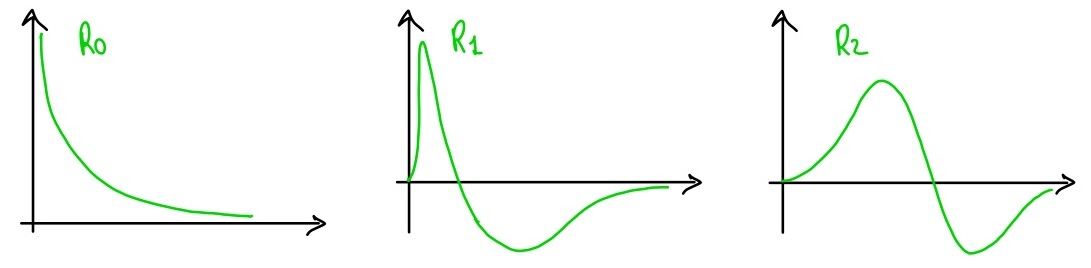
\includegraphics[scale=0.30]{img_5}
	\caption{Representation of s-waves}
	\label{fig_swaves}
\end{figure}
\textbf{N.B.}: defining $U(r) \equiv rR(r)$ implies
\[
-\frac{\hbar}{2m} \frac{d^2}{dr^2} U(r) + \frac{\hbar l(l+1)}{2mr^2} U(r) - \frac{e^2}{r} u(r) = E U(r)
\]
Where $u(r)$ is not a potential. When we tried to solve the h-atom with classical mechanics, the analogy with the kinetic energy was perfect. This is not quite the case?
Finally we want to calculate the probability of a particle to be at distance $r$.
\[
drProb(r)=|R(r)|^2r^2dr
\]
\[
P(\vec{r},\vec{r}+dr)=\int_{\vec{r}}^{\vec{r}+dr}dr\,r^2\iint d\theta\,d\varphi\,|R(r)\,Y(\theta,\varphi)|^2=\int_{\vec{r}}^{\vec{r}+dr}dr\,r^2R^2(r)\iint_{sph}\,d\theta\,d\varphi|Y|^2
\]
Since the function is not dependent on $\theta$ or $\varphi$, the integral equals 1.
\[
P(\vec{r},\vec{r}+dr)=\vec{r}^2R^2(r)dr
\]
Depending on the value of $l$ I can get the probability of the electron depending on $\theta$ and $\varphi$. At $l=0$ the probability is more concentrated on the centre and then fades out (s orbital). At $l=1$ the function depends on $\theta$ but not on $\varphi$, the function is cylindrically symmetrical (p orbital). It is important to remember that there is no orbit in an atom, for the concept of trajectory breaks down on a quantum level.\\
\\

\section{Relationship between spin and statistics: Quantum many-body systems}
\subsection{The importance of spin}
Spin statistics can explain chemistry, quantum entanglement, and quantum computers.\\
Stern Gerlach experiments confirm the fact that electrons have a magnetic moment, which is quantised in integers or half integers, because they can interact with a magnetic field. Generally, particles behave differently and may have different states of being.\\
What we know is that we cannot measure more than one component of the magnetic moment (quantum uncertainty) and this \textbf{intrinsic} magnetic moment behaves like an angular momentum.\\
The rotation of the electron upon itself generates a magnetic field and a magnetic moment. This is called \textbf{spin}, $\hat{S^2},\hat{S_z}$ a property of particles that \textbf{doesn't change with time} and that can distinguish a particle from one another.\\
\newline
We assume that:
\[ [\hat{S_x}\,,\,\hat{S_y}]=i\hbar\hat{S_z} \]
\[ [\hat{S_z}\,,\,\hat{S^2}]=\hat{0} \]
The values of $\hat{S^2}$ characterize the behaviour of the particle.\\
\[\hat{L^2}\,\rightarrow\,l=0, 1, 2, ...\]
\[\hat{S^2}\,\rightarrow\,s=0, \frac{1}{2}, 1, \frac{3}{2}, ...\]
Electrons, neutrons, and protons have $s=1/2$. Photons, for instance, have $s=1$.\\

\subsection{Spin-Statistics theorem for identical particles}
Let's consider a wave function of many identical particles $\psi$, for instance $n$ identical electrons with spin $s$, $\hat{S_z}$, and position $r$. All the particles have the same velocity.\\
\[
\Psi(\vec{r_1}, s_1^z, \vec{r_2}, s_2^z, ..., \vec{r_n}, s_n^z) \text{   ,with } \vec{q}=(\vec{r},\vec{s_z})
\]
\[\text{For identical particles: }\Psi(\vec{q_1},\vec{q_2}, ..., \vec{q_n})A[\Psi(\vec{q_1},\vec{q_2}, ..., \vec{q_n})\pm\Psi(\vec{q_1},\vec{q_2}, ..., \vec{q_n})] \]
\textbf{Antisymmetric wave-function (fermions)}: wave-function that under the exchange of pairs of identical particles has a total spin, $s$, that is an \textbf{half integer} (1/2, 3/2, ...). Swapping the wave function \textbf{changes} it.\\
\[\Psi(\vec{q_1},\vec{q_2}, ..., \vec{q_n})=-\Psi(\vec{q_1},\vec{q_2}, ..., \vec{q_n})\]
The particles that have an antisymmetric wavefunction are called \textbf{fermions}.\\
\newline
\textbf{Symmetric wave-function (bosons)}: wave function that under the exchange of pairs of identical particles has a total spin, $s$, that is an \textbf{integer} (1, 2, 3, ...). Swapping the wave function \textbf{doesn't change} it.\\
\[\Psi(\vec{q_1},\vec{q_2}, ..., \vec{q_n})=\Psi(\vec{q_1},\vec{q_2}, ..., \vec{q_n})\]
The particles that have a symmetric wavefunction are called \textbf{bosons}.
\begin{quote}
	"A fermion once, a fermion forever".\\
	"Fermions and bosons are like Montecchi and Capuleti. They don't want anything to do with each other"\\
	- Pietro Faccioli
\end{quote}
\noindent
\textbf{Corollary}: In a quantum wave function, there cannot be two fermions with identical state or else two identical fermions cannot be found in the same quantum state.
\[\Psi(q_1, q_2)= -\Psi(q_2,q_1)\] the two electrons are the same, $q_1=q_2=q$
\[\Psi(q,q)=-\Psi(q,q) \]
The only condition for which this equality is true is for  $\Psi = 0$, there is no wave function that can describe a system of two identical fermions with identical state. This is called \textbf{Pauli's exclusion principle} and applies to all identical fermions.
\\
\subsection{Mean Field Approximation}
Solving the S.E. for more than one particle rapidly becomes challenghing, even resorting to High Performance Computing. However, much of the global, qualitative structure of the Mondelyev table can be understood within a simple \textbf{mean field} picture: instead of accounting for all pairwise Coulomb interactinos, we assume that the effect on each electron, due to all other electrons and the protons can be represented by an overall confining potential.\\
Suppose we are dealing with two electrons:
\[
\bigg(-\frac{\hbar^2}{2m}\sum_{i}^{N}\nabla^2_i+U(\vec{r_1}...\vec{r_n})\bigg)\Psi(\varphi_1 ... \varphi_n)=E\Psi(q_1 ... q_n)
\]
The solution to the eigenvalue problem that is also antisymmetric to the potential depends on the position.
\[
U(\vec{r_1}...\vec{r_n})=\sum_{i,j}\frac{e^2}{|\vec{r_i}-\vec{r_j}|}-e^2\frac{\mathbb{Z}}{r_i}
\]
Instead of keeping track of all the interactions of particles on one another, we consider the average of the whole many-body system, e.g., mean coulombic repulsion. I calculate the interaction between single electron and average electron density. The larger symmetry is the ground state, which for the H-atom this is \textbf{1s}, as shown in figure \ref{fig:spin1}.\\
\begin{figure}[htbp!]
	\centering
	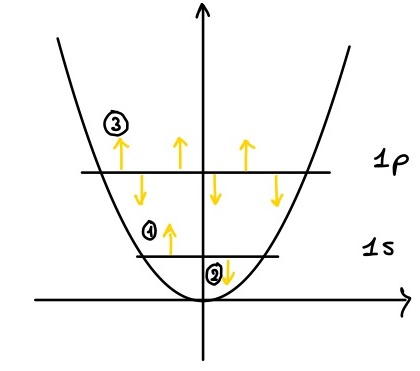
\includegraphics[scale=0.20]{img_6}
	\caption{Position of electrons in the 1p and 1s states with relative spin (up pr down)}
	\label{fig:spin1}
\end{figure}
\\
The structure of the wave function is influenced by spin even if it doesn't appear in the hamiltonian and can be used not only for electrons but for all subatomic/subnuclear particles. \\
We may ask ourselves: is there any stable nucleus? For clarity, a nucleus is divided into two different type of nucleons, protons and neutrons. Nucleons can have two different states: spin up (protons) and spin down (neutrons). Actually, the spin is really the only thing that allow us to differentiate the two, since their mass is basically the same (neutrons have a little heavier mass). For each spin there's an isospin up and an isospin down (isospin measures the charge). An example of (impossible) nucleus decay is shown in figure \ref{fig:decay}.\\
\begin{figure}[htbp!]
	\centering
	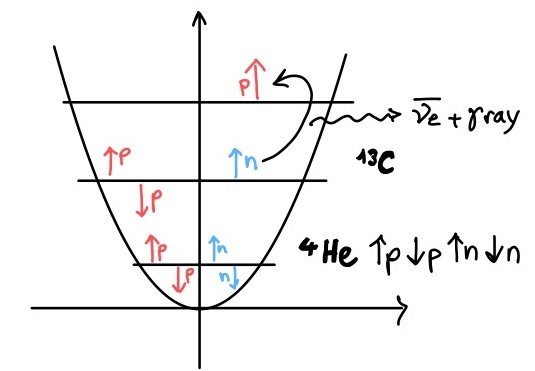
\includegraphics[scale=0.20]{img_7}
	\caption{In this picture the $He^4$ nucleus is represented. It it the most stable nucleus ($\alpha$particle). The thing is that the difference in mass ($m_n > m_p$) $\Delta m \rightarrow \text{energy}$ is not sufficient to reach the higher energy state and become a proton. Is there any other way? No, because of the spin theory. So, even if in principle a neutron could decay into a proton, ultimately Pauli's exclusion principle does not allow to have the same spin.}
	\label{fig:decay}
\end{figure}\\


\subsection{Quantum Entanglement}
In an external/mean potential, the Schr\"odinger equation has a potential of a single coordinate that depends on where that potential is located, thanks to the mean field approximation.
\[
\hat{H}=-\frac{\hbar^2}{2m}\sum_{i}\nabla_i^2+\sum_{i=1}^NU(q_i)=\sum_i h_i
\]
When $\hat{H}$ is separable into two parts, the wave function is the product of these two parts.\\
Consider N identical spin-0 bosons (simplest system that represents the sum of all possible permutations for N > 2):\\
\[
\Psi(r_1, ..., r_n)= \prod_K^n\varphi_n(r_i)=\varphi_1(r_1)\cdot ... \cdot \varphi_n(r_n)
\]
If I swap two excited states eg., $\varphi_s(r_3)$ and $\varphi_p(r_1)$, I do not obtain the same wave function (I get $\varphi_s(r_1)$ and $\varphi_p(r_3)$) so they are antisymmetric. If I swap two ground states they stay the same (they are symmetric). This system is also used for distinguishable particles (boltzmanions) or identical particles in semiclassic regimes.\\
\newline
Consider now two identical fermions described by single-electron wave functions.\\
\[
\Psi(r_1, s_1^2, r_2, s_2^2)=\varphi_{\uparrow}(r_1)\varphi_{\downarrow}(r_2)
\]
We can prove that the wave function of the two different fermions (hence each one is described by a different spin state) system is antisymmetric. This is called \textbf{Slater determinant} for N>2 fermions.
\[
\Psi=\frac{1}{\sqrt{2}}\big(\varphi_{\uparrow}(r_1)\varphi_{\downarrow}(r_2)+\varphi_{\uparrow}(r_2)\varphi_{\downarrow}(r_1)\big)
\]
by swapping their indices
\[
\Psi'=\frac{1}{\sqrt{2}}\big(\varphi_{\uparrow}(r_2)\varphi_{\downarrow}(r_1)-\varphi_{\uparrow}(r_1)\varphi_{\downarrow}(r_2)\big)
\]
and it's noticeable how $\Psi = -\Psi'$. The two functions are antisymmetric.\\
This represents a quantum superposition of states. In order to follow Pauli's principle, each state has a 50\% of probability to occur and when $r_1$ is $\uparrow$,  $r_2$ must necessarily be $\downarrow$. We found out that Pauli's principle \textbf{entangles}particles. In our case with two fermions, the state of particle n.2 is entangled to the state of particle 1.

\begin{center}
\textbf{Quantum entanglement}: a physical phenomenon that occurs when a group of particles are generated, interact, or share spatial proximity in a way such that the quantum state of each particle of the group cannot be described independently of the state of the others, including when the particles are separated by a large distance.
\end{center}

The two particles are said to be an \textbf{EPR pair} (Einstein-Podolsky-Rosen) and the state of the two particles is called a \textbf{Bell state}.
If I measure spin 1, the wave function collapses into spin value 1 and spin 2 consequently collapses into spin value 2.\\
The concept of \textbf{quantum entanglement} has no correspondences in classical mechanics and is used to develop quantum computers.\\
In classical computers the iformation is carried on in one single state out of two (either the gate is open or is closed, binary system). In quantum computers I have N states, I have $2^N$ states entangled with each other at the same time. I can store much more information in $2^N$ compared to 1 \footnote{It may confuse a little, beacause we know that in a classical architecture, N bits can represent $2^N$ numbers. This formulation is not very correct and I will provide my own understanding on the matter. That is, with N bits we can ultimately have just one number, even if we have N possible ways to arrange the bits. Instead, a quantum architecture supports $2^N$ states \textit{simultaneously}. This more expressive power contributes to the idea of "quantum supremacy".}. \\
\newline
The antisymmetric equation is the determinant of this matrix:
\[
\frac{1}{\sqrt{2}}
\begin{pmatrix}
\varphi_1(r_1)&\varphi_2(r_1)\\
\varphi_1(r_2)&\varphi_2(r_2)
\end{pmatrix}
\]
that can be generalized into
\[
\frac{1}{\sqrt{2}}
\begin{pmatrix}
\varphi_1(r_1)&...&\varphi_n(r_1)\\
... & &...\\
\varphi_1(r_m)&...&\varphi_n(r_m)
\end{pmatrix}
\]
This latter matrix is called \textbf{Slater matrix} and I can calculate Slater determinant that guarantees that the wave function is antisymmetric.\\

\subsection{Mathematical formalism of Stern-Gerlach experiment}
The spin $\hat{S^2}$ doesn't have a classical correspondence, we cannot directly obtain a formula for $\hat{S^2}$ in classical mechanics. I must find objects that have two states.\\
Consider spin $1/2$ only and choose an Hillbert space and an operator that acts on it. Since a particle with $s=1/2$ can have two different states, the most natural choice for a Hillbert space would be \emph{$L^2$}.\\
The eigenstates of the z-components are:
\[\ket{\uparrow}=\begin{pmatrix}1\\0\end{pmatrix}\, \ket{\downarrow}=\begin{pmatrix}0\\1\end{pmatrix}\]
$\hat{S_x}$, $\hat{S_y}$, and $\hat{S_z}$ are represented by 2x2 matrices that must obey the commutation rule of $[\hat{S^2}\,,\,\hat{S_z}]=0$ and $[\hat{S_x}\,,\,\hat{S_y}]=i\hbar\hat{S_z}$.
\\
\textbf{Pauli matrices:}
\[
\hat{S_x}=\frac{\hbar}{2}\begin{pmatrix}0&1\\1&0\end{pmatrix}\;\,
\hat{S_y}=\frac{\hbar}{2}\begin{pmatrix}0&-i\\i&0\end{pmatrix}\;\,
\hat{S_z}=\frac{\hbar}{2}\begin{pmatrix}1&0\\0&-1\end{pmatrix}
\]
The normalized eigenstates for the x-component are:
\[
\ket{\rightarrow}=\frac{1}{\sqrt{2}}\begin{pmatrix}1\\1\end{pmatrix}\;\,
\ket{\leftarrow}=\frac{1}{\sqrt{2}}\begin{pmatrix}1\\-1\end{pmatrix}\,
\]
We can find the conditional probability of finding spin up with the condition of being in a state of spin left (but also spin up given spin up, etc.).
\[
P(\ket{\uparrow}|\ket{\leftarrow})=\bigg(\frac{1}{\sqrt{2}}\begin{pmatrix}1&0\end{pmatrix}\begin{pmatrix}1\\-1\end{pmatrix}\bigg)^2=\frac{1}{2}
\]
\[
P(\ket{\uparrow}|\ket{\uparrow})=\bigg(\frac{1}{\sqrt{2}}\begin{pmatrix}1&0\end{pmatrix}\begin{pmatrix}1\\0\end{pmatrix}\bigg)^2=1
\]
\[
P(\ket{\leftarrow}|\ket{\uparrow})=\bigg(\frac{1}{\sqrt{2}}\begin{pmatrix}1&-1\end{pmatrix}\begin{pmatrix}1\\0\end{pmatrix}\bigg)^2=\frac{1}{2}
\]
This is also the mathematical formalism that represents the Stern Gerlach experiment. In fact, if we calculate $P(\ket{\uparrow}|\ket{\leftarrow}) = \frac{1}{2}$, then $P(\ket{\uparrow}|\ket{\uparrow}) = 1$, we will get again $P(\ket{\uparrow}|\ket{\leftarrow}) = \frac{1}{2}$.  \\
We can calculate $\hat{S^2} = \hat{S_x}^2+\hat{S_y}^2+\hat{S_z}^2$ that results in a sum of identity matrices, in fact
\[\hat{S^2}=\frac{3}{4}\hbar^2\big(\mathds{1}_e\big)\]
The identity matrix $\\mathds{1}_e$ allows $\hat{S^2}$ to commute with every component of the spin operator.

\subsection{Tensor product states}
Up until now, we learned how to deal with spin's degrees of freedom only. But how do we integrate spin in the $L_2$ space of the wave function? We'll use the tensor product. Given two vectors, the definition of tensor product is:
\[
\begin{pmatrix}a_1\\a_2\\...\\a_n\end{pmatrix}\otimes\begin{pmatrix}b_1\\b_2\\...\\b_n\end{pmatrix}=\begin{pmatrix}a_1b_1\\a_1b_2\\...\\a_1b_n\\a_2b_1\\a_2b_2\\...\\a_mb_n\end{pmatrix}
\]
Tensor product is obtained by multiplying each $a$ term with every $b$ term. It creates another vector space (a larger Hillbert space) that is used to combine spins for many particles, spin and particle space of one particle ect.\\
Tensor product is used to describe the \emph{combination of two quantum states}.
\[\text{Quantum state of particle 1: } \begin{pmatrix}\alpha_1\\\alpha_2\end{pmatrix}=\alpha_1\begin{pmatrix}1\\0\end{pmatrix}+\alpha_2\begin{pmatrix}0\\1\end{pmatrix}=\alpha_1\ket{\uparrow}+\alpha_2\ket{\downarrow}=\vec{\ket\alpha}\]
\[\text{Quantum state of particle 2: } \begin{pmatrix}\beta_1\\\beta_2\end{pmatrix}=\beta_1\begin{pmatrix}1\\0\end{pmatrix}+\beta_2\begin{pmatrix}0\\1\end{pmatrix}=\beta_1\ket{\uparrow}+\beta_2\ket{\downarrow}=\vec{\ket{\beta}}\]
These two single quantum states represent qubits.\\
\[\text{Combination of the two states: }
\vec{\ket{\alpha}}\otimes\vec{\ket{\beta}}\equiv{\ket{\vec{\alpha}\vec{\beta}}}=\begin{pmatrix}\alpha_1\beta_1\\\alpha_1\beta_2\\\alpha_2\beta_1\\\alpha_2\beta_2\end{pmatrix}
\]
The combination of the two states creates a wavefunction which amplitude corresponds to the observation of all the combinations of the particles. For example, $\alpha_1\,\beta_1$ is the amplitude of observing the first particle $\uparrow$ and the second particle $\uparrow$ \\
We can build the basis for a vector product of two particles and with this we can describe four different states since $\mathbb{R}^2\otimes\mathbb{R}^2=\mathbb{R}^4$
\[
\begin{pmatrix}1\\0\\0\\0\end{pmatrix}=\ket{\uparrow\uparrow}\begin{matrix}\alpha_1=1\\\beta_1=1\end{matrix}\bigg| \;\;
\begin{pmatrix}0\\1\\0\\0\end{pmatrix}=\ket{\uparrow\downarrow}\begin{matrix}\alpha_1=1\\\beta_2=1\end{matrix}\bigg| \;\;
\begin{pmatrix}0\\0\\1\\0\end{pmatrix}=\ket{\downarrow\uparrow}\begin{matrix}\alpha_2=1\\\beta_1=1\end{matrix}\bigg| \;\;
\begin{pmatrix}0\\0\\0\\1\end{pmatrix}=\ket{\downarrow\downarrow}\begin{matrix}\alpha_2=1\\\beta_2=1\end{matrix}\bigg|
\]
We can also derive the most general quantum mechanical state description of the EPR pair:
\[
\ket{\vec{\alpha}\vec{\beta}}=\alpha_1\beta_1\ket{\uparrow\uparrow}+\alpha_1\beta_2\ket{\uparrow\downarrow}+\alpha_2\beta_1\ket{\downarrow\uparrow}+\alpha_2\beta_2\ket{\downarrow\downarrow}
\]
In this way I can carry on information about multiple state simultaneously.\\
\newline
Given $\varphi(x)$ wavefunction lives in a \emph{$L^2$} Hillbert space.\\
\[
\varphi(x)\otimes(\alpha\ket{\uparrow}+\beta\ket{\downarrow})=\begin{pmatrix}\alpha\varphi(x)\\\beta\varphi(x)\end{pmatrix}=\begin{pmatrix}\varphi_{\uparrow}(x)\\\varphi_{\downarrow}(x)\end{pmatrix}
\]
This latter matrix is called a \textbf{spinor}, which is a wavefunction that includes spin amplitude (usually wavefunction doesn't have information about spin of the particle).\\
Let's consider a \underline{non-entangled state}.
\[
\ket{\Psi}=\frac{1}{\sqrt{2}}\ket{\uparrow\uparrow}+\frac{1}{\sqrt{2}}\ket{\uparrow\downarrow}=\ket{\alpha\uparrow}
\]
The two measures are independent of each other, I can find particle 2 with a probability which is independent of the measurement of particle 1. It is said to be factorizable.\\
Let's now consider an \underline{entangled state}:
\[
\ket{\Psi}=\frac{1}{\sqrt{2}}\big(\ket{\uparrow\downarrow}+\ket{\downarrow\uparrow}\big) = \begin{pmatrix}0\\\frac{1}{\sqrt{2}}\\\frac{1}{\sqrt{2}}\\0\end{pmatrix}
\]
Note that the expression cannot be factorized now. We can generate an operator that generates entangled states:
\[
\frac{\big(\ket{\uparrow\downarrow}+\ket{\downarrow\uparrow}\big)}{\sqrt{2}}=\frac{1}{\sqrt{2}}\begin{pmatrix}0\\1\\1\\0\end{pmatrix}\bigg(U\bigg)\begin{pmatrix}1\\0\\0\\0\end{pmatrix}
\]
U is called \textbf{quantum gate} in quantum computing.\\
Quantum gates can be defined as a \textbf{time evolution operators} that acts on the function to solve time-dependent Schr\"odinger equation and provide the dynamics of the system.\\
$\hat{U}(\Delta t) = e^{i\hat{H}\Delta t}$ at state $\ket{\Psi(0)}$ can be approximated with $(1-\hat{H}\Delta t)$ and this latter can be solved by a quantum gate to give out $\ket{\Psi(t)}$. This operation cannot be solved by classical computers, dynamics is naturally given out by quantum computers.\\

\textit{Example: A three-electrons system}
Remember that thanks to the mean field approximation (nedeed for many-body calculations) we have the advantage that:
\[
\sum_{i<j} U(r_{ij}) \simeq \sum_i \bar{U}(r_i)
\]
making the computation piece-wise and therefore, muche easier to solve.
The Hamiltonian becomes the sum of many small hamiltonians:
\[
H = \sum_{ij} h_i \rightarrow \phi(q_1, ... , q_n) = \prod_i \phi(q_i)
\]
with $q_i = (\bar{r}_i, S^z_i)$ representing the position. The thing is that a simple product generally does not respect the spin and its rules (e.g. Pauli blocking). This factorization works well for distinguishable particles, like in Boltzmanions systems. These are almost classical settings. \\
Let's assume we have he following systems:
\[
\textbf{Bosons} \;\; \frac{1}{\sqrt{2}}(\phi_0(r_1)\phi_1(r_2) + \phi_0(r_2)\phi_1(r_1))
\]
\[
\textbf{Fermions} \;\; \frac{1}{\sqrt{2}}(\phi_0(r_1)\phi_1(r_2) + \phi_0(r_2)\phi_1(r_1))
\]
While for bosons for systems with $N>2$ the sum of permutations is sufficient (symmetry), for fermions we'll need to calculate the Slater determinant (since it's guaranteed that the wave-function is antisymmetric). \\
For this application ($N = 3 $) we need two energy levels. Indeed if we try to force the three particles in the same s-state, the Slater determinant will eventually go to zero.\\
\[
\det\frac{1}{\sqrt{N!}}
\begin{pmatrix}
\phi_s^\uparrow(r_1)&\phi_s^\uparrow(r_2)&\phi_s^\uparrow(r_3)\\
\phi_s^\downarrow(r_1)&\phi_s^\downarrow(r_2)&\phi_s^\downarrow(r_3)\\
\phi_p^\uparrow(r_1)&\phi_p^\uparrow(r_2)&\phi_p^\uparrow(r_3)\\
\end{pmatrix}=
\]
\[
=\frac{1}{\sqrt{N!}}\big[
\phi_s^\uparrow(r_1)\phi_s^\downarrow(r_2)\phi_p^\uparrow(r_3)
-\phi_s^\uparrow(r_1)\phi_s^\downarrow(r_3)\phi_p^\uparrow(r_2)
-\phi_s^\uparrow(r_2)\phi_s^\uparrow(r_3)\phi_p^\uparrow(r_1)\]
\[+\phi_s^\uparrow(r_2)\phi_s^\downarrow(r_1)\phi_p^\uparrow(r_3)
+\phi_s^\uparrow(r_3)\phi_s^\downarrow(r_1)\phi_p^\uparrow(r_2)
-\phi_s^\uparrow(r_3)\phi_s^\downarrow(r_2)\phi_p^\uparrow(r_1)
\big]
\]
Six-terms determinant, complicated to evaluate!\\
\newline
\textit{Example: Application of the mean field approximation to calculate the density of electrons in a point ($N=2$)}\\
\newline
We can define a \textit{density operator}
\[
\hat{\rho}(x)=\sum_i\delta(x-r_i)
\]
and apply it to a wave function that defines a point with two electrons (basically we want to calculate how much space these electrons occupy). We want to calculate $\mel{\Psi}{\hat{\rho}(x)}{\Psi}$
The wave function is:
\[
\Psi(\vec{r_1},\vec{r_2},s_1^z,s_2^z)=\frac{1}{\sqrt{2}}\big(\phi_\uparrow(r_1)\phi_\downarrow(r_2)-\phi_\downarrow(r_1)\phi_\uparrow(r_2)\big)
\]
\marginpar{\textit{This is a 6-dim integral}}
\[
\mel{\Psi}{\hat{\rho}(x)}{\Psi}=\frac{1}{2}\int d\vec{r_1}d\vec{r_2} \Psi^*(\vec{r_1},\vec{r_2},s_1^z,s_2^z)\cdot\bigg(\sum_i \delta(\vec{x}-\vec{r_i})\bigg)\cdot\Psi(\vec{r_1},\vec{r_2},s_1^z,s_2^z)=
\]
\[
=\frac{1}{2}\int d\vec{r_1}d\vec{r_2}\big(\phi^*_\uparrow(r_1)\phi^*_\downarrow(r_2)-\phi^*_\downarrow(r_1)\phi^*_\uparrow(r_2)\big)\cdot\big(\delta(\vec{x}-\vec{r_1})+\delta(\vec{x}-\vec{r_2})\big)\cdot\big(\phi_\uparrow(r_1)\phi_\downarrow(r_2)-\phi_\downarrow(r_1)\phi_\uparrow(r_2)\big)
\]
\[
=\frac{1}{2}\int_1\int_2\bigg[
\phi_1^{*\uparrow}\phi_2^{*\downarrow}\delta_1\phi_1^\uparrow\phi_2^\downarrow
+\phi_1^{*\uparrow}\phi_2^{*\downarrow}\delta_2\phi_1^\uparrow\phi_2^\downarrow
-\phi_1^{*\uparrow}\phi_2^{*\downarrow}\delta_1\phi_2^\uparrow\phi_1^\downarrow
-\phi_1^{*\uparrow}\phi_2^{*\downarrow}\delta_2\phi_1^\downarrow\phi_2^\uparrow -\]
\[
-\phi_1^{*\downarrow}\phi_2^{*\uparrow}\delta_1\phi_1^\uparrow\phi_2^\downarrow
-\phi_1^{*\downarrow}\phi_2^{*\uparrow}\delta_2\phi_1^\uparrow\phi_2^\downarrow
+\phi_1^{*\downarrow}\phi_2^{*\uparrow}\delta_1\phi_1^\downarrow\phi_2^\uparrow
+\phi_1^{*\downarrow}\phi_2^{*\uparrow}\delta_2\phi_1^\downarrow\phi_2^\uparrow
\bigg]d\vec{r_1}d\vec{r_2}
\]
Now note that when the operator acts, e.g., on the electron 1, the remaining $\int \phi_2^{*\uparrow}\phi_2^\uparrow d\vec{r_2}=1$
\[
=\frac{1}{2}\int \phi_1^{*\uparrow}\phi_1^\uparrow \,\delta_1\, d\vec{r_1}
+\int \phi_2^{*\downarrow}\phi_2^\downarrow\, \delta_2\, d\vec{r_2}
-\int \phi_1^{*\uparrow}\phi_1^\downarrow d\vec{r_1}
-\int \phi_2^{*\downarrow}\phi_2^\uparrow d\vec{r_2}-\]
\[
-\int \phi_1^{*\downarrow}\phi_1^\uparrow d\vec{r_1}
-\int \phi_2^{*\uparrow}\phi_2^\downarrow d\vec{r_2}
+\int \phi_1^{*\downarrow}\phi_1^\downarrow\, \delta_1\, d\vec{r_1}
+\int \phi_2^{*\uparrow}\phi_2^\uparrow\, \delta_2\, d\vec{r_2}
\]
We can recall the fact that by construction $\phi_1^{*\uparrow}\phi_1^\uparrow=|\phi_1^\uparrow|^2$  and this $|\phi_1^\uparrow|^2$ corresponds to the probability of finding electron 1 with spin $\uparrow$ ($P^\uparrow(x)$). Same applies to electron 2.\\
\[
=\frac{1}{2}\int |\phi_1^\uparrow|^2 \,\delta_1\, d\vec{r_1}
+\int |\phi_2^\downarrow|^2\, \delta_2\, d\vec{r_2}
-\int \phi_1^{*\uparrow}\phi_1^\downarrow d\vec{r_1}
-\int \phi_2^{*\downarrow}\phi_2^\uparrow d\vec{r_2}-\]
\[
-\int \phi_1^{*\downarrow}\phi_1^\uparrow d\vec{r_1}
-\int \phi_2^{*\uparrow}\phi_2^\downarrow d\vec{r_2}
+\int |\phi_1^\downarrow|^2\, \delta_1\, d\vec{r_1}
+\int |\phi_2^\uparrow|^2\, \delta_2\, d\vec{r_2}
\]
The integrals with an electron present with opposite spins $\int \phi_1^{*\uparrow}\phi_1^\downarrow d\vec{r_1}$ (aka the integrals with negative signs) represent the probablity of finding the particle in state $\uparrow$ \textbf{and} $\downarrow$ that is zero, so they cancel. Mind that the contribution from the entanglement of the two states doesn't occur within observables so the inner product is zero. Fermions, though, must be entangled to give an antisymmetric wavefunction.\\
By knowing that $\int\,dx\, g(x)\delta(x-x_0)=g(x_0)$ and by considering that there's no point in distinguishing the two electrons for anything but their spins (they have same mass and charge), we can say that:
\[P_1^\uparrow(x)=P_2^\uparrow(x)=P^\uparrow(x)\]
\[P_1^\downarrow(x)=P_2^\downarrow(x)=P^\downarrow(x)\]
Hence the probability density becomes
\[
\mel{\Psi}{\hat{\rho}(x)}{\Psi}=\frac{1}{2}\bigg[P^\uparrow(x)+P^\uparrow(x)+P^\downarrow(x)+P^\downarrow(x)\bigg]=P^\uparrow(x)+P^\downarrow(x)
\]
Either a particle is spin up or spin down in $x$.
